\chapter{PORTAFOLIO DE GESTIÓN DEL PROYECTO}
\label{anx:portafolio}

El portafolio del proyecto se conserva en \RepoProyecto, organizado en las carpetas siguientes:
\begin{itemize}
\item \enlacerepo{informe}: fuente \LaTeX{} y versiones en PDF de este informe;
\item \enlacerepo{cfd}: casos de ANSYS Fluent y OpenFOAM, guiones de posproceso y tablas de resultados del modelo de mojado;
\item \enlacerepo{hidraulica}: guiones y resultados de las redes de 19, 22 y 24 boquillas, y esquema hidráulico;
\item \enlacerepo{estructural}: modelos de SAP2000, modelos de CalculiX, cálculo de las uniones y libro mecánico del soporte;
\item \enlacerepo{cad}: modelo FreeCAD integrado, planos de SolidWorks y estudios complementarios;
\item \enlacerepo{gestion}: diagrama de Gantt, actas de las reuniones con el asesor y registro de decisiones de diseño.
\end{itemize}

El registro de decisiones guarda, para cada decisión, la fecha, las alternativas consideradas, la razón, la evidencia y su estado.

\section{Cronograma del proyecto}
\label{sec:cronograma-proyecto}

El segundo curso de Proyecto Final de Ingeniería se planificó en dieciséis semanas, del 10 de agosto al 29 de noviembre de 2026, en cuatro fases cerradas por un entregable: definición y contexto (primer entregable, 13 de septiembre), Caso Base y simulación (segundo entregable, 11 de octubre), iteración y rediseño (informe final, 22 de noviembre) y sustentación (29 de noviembre). La Figura~\ref{fig:gantt-1} presenta las fases 1 y 2 del cronograma, y la Figura~\ref{fig:gantt-2}, las fases 3 y 4.

\begin{figure}[p]
\centering
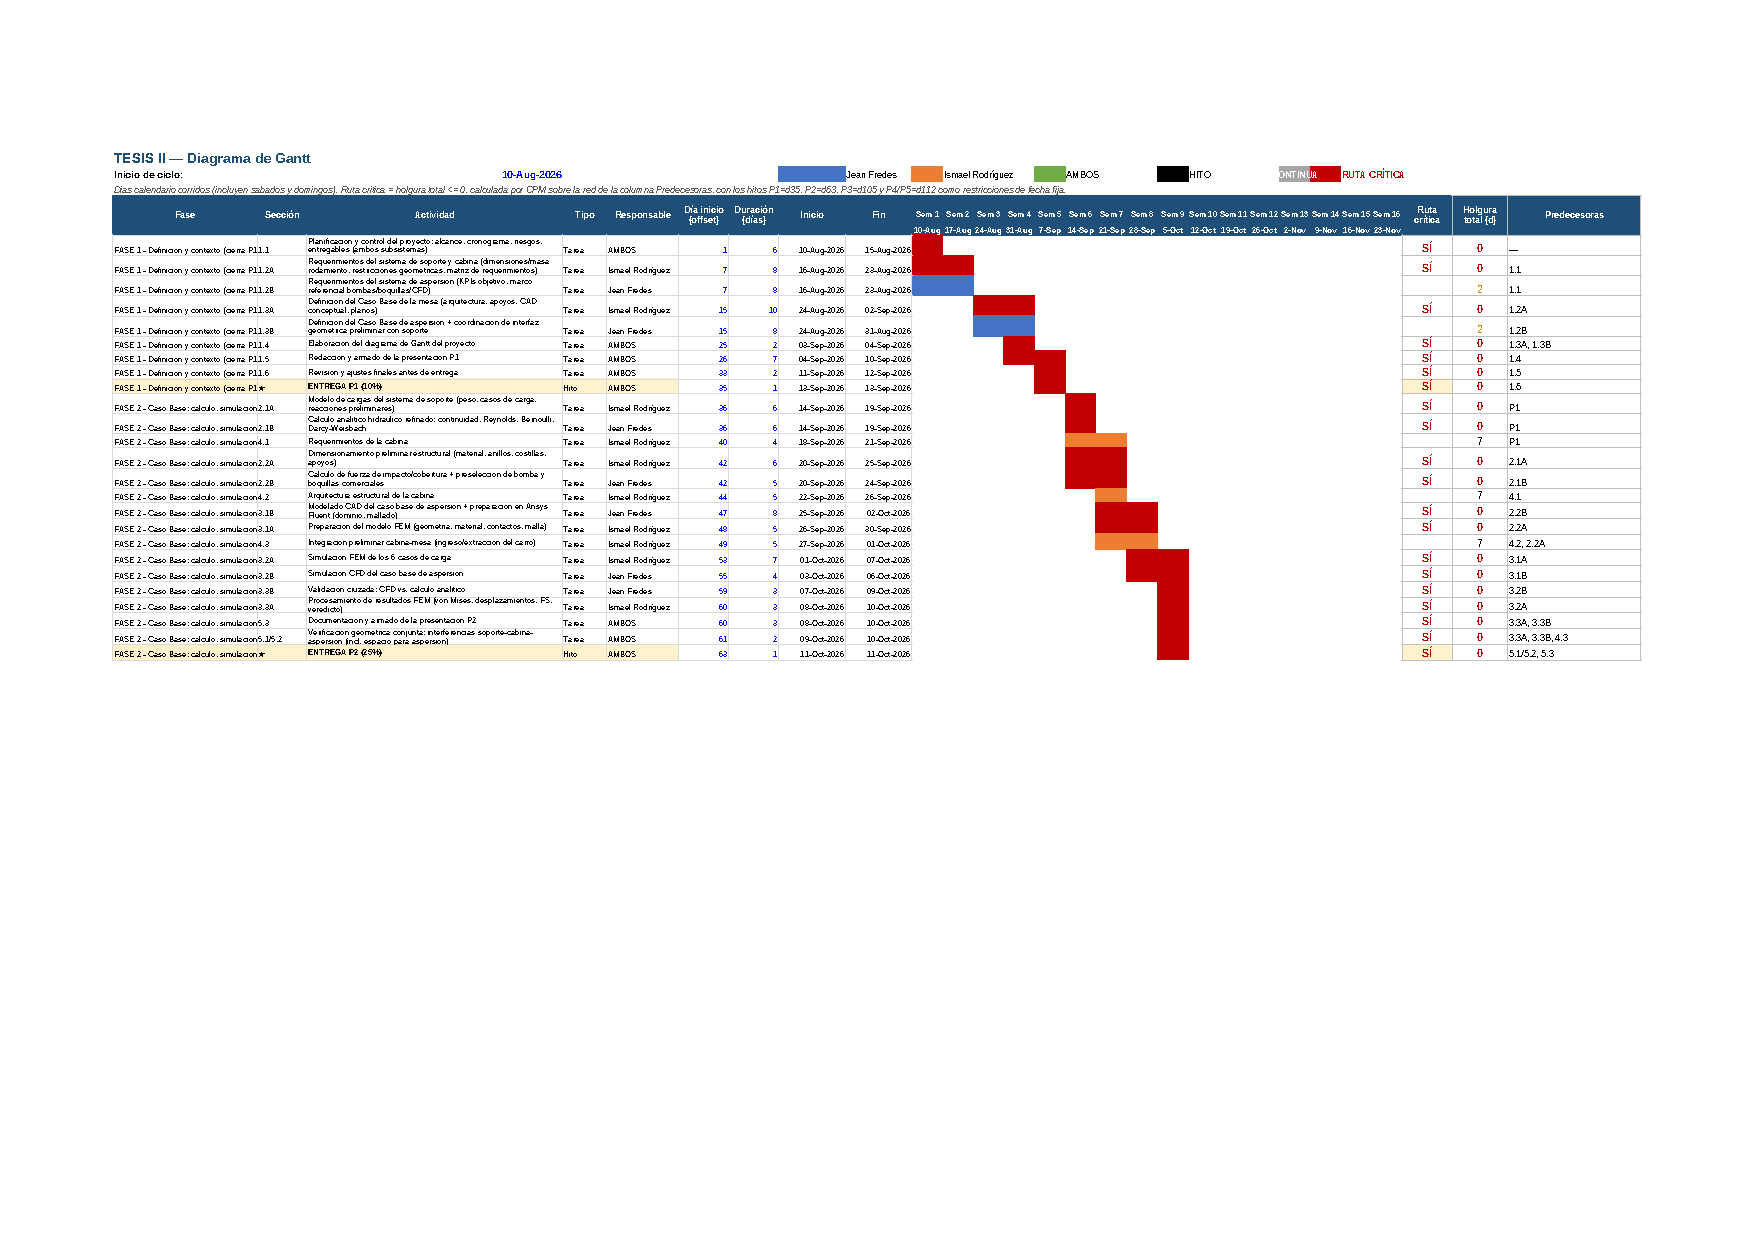
\includegraphics[page=1,trim=50bp 274bp 50bp 68bp,clip,angle=90,height=0.86\textheight]{anexos/Anexo_Gantt_TesisII.pdf}
\caption{Diagrama de Gantt del proyecto: fases 1 y 2 (10/08/2026--11/10/2026). Elaboración propia.}
\label{fig:gantt-1}
\end{figure}

\begin{figure}[p]
\centering
\includegraphics[page=2,trim=50bp 251bp 50bp 68bp,clip,angle=90,height=0.86\textheight]{anexos/Anexo_Gantt_TesisII.pdf}
\caption{Diagrama de Gantt del proyecto: fases 3 y 4 (12/10/2026--29/11/2026). Elaboración propia.}
\label{fig:gantt-2}
\end{figure}
